\section{Methodology}
%short introduction about CFD and the usage of ansys fluent
To understand the flow behaviour of various undertray geometry, fluid dynamics analysis is required. The rapid development of computational power has allowed more accurate and reliable results in computational analysis such as computational fluid dynamics (CFD)\cite{Andersson2011ComputationalEngineers}. The usage of CFD allows engineers to simplify the processes and achieve an accurate result in shorter time which allows engineers to do more iterations. 

\noindent The methodology consists of 3 phase which are 2D enclosed \& open-flow, 3D bluff body, 3D undertray. The first phase is the 2D analysis which analyse the undertray variables on a Venturi-tube like geometry and open-flow analysis analyse a simple bluff body with similar undertray variables. 3D bluff body will take the 2D geometry and extrude it as an 3D geometry which then analysed with the same undertray variables. Lastly is the 3D undertray where the optimised results from previous analysis will be used to determine the geometry of the final undertray design. To achieve realistic results, simplified traced body from the QFR 2021 car will be attached to the undertray. The process flow can be illustrated on figure \ref{fig:project methodology}. The work on this paper will be fully based on CFD which utilise ANSYS Fluent as a default working platform.

\begin{figure}[ht!]
    \centering
    \makebox[\textwidth]{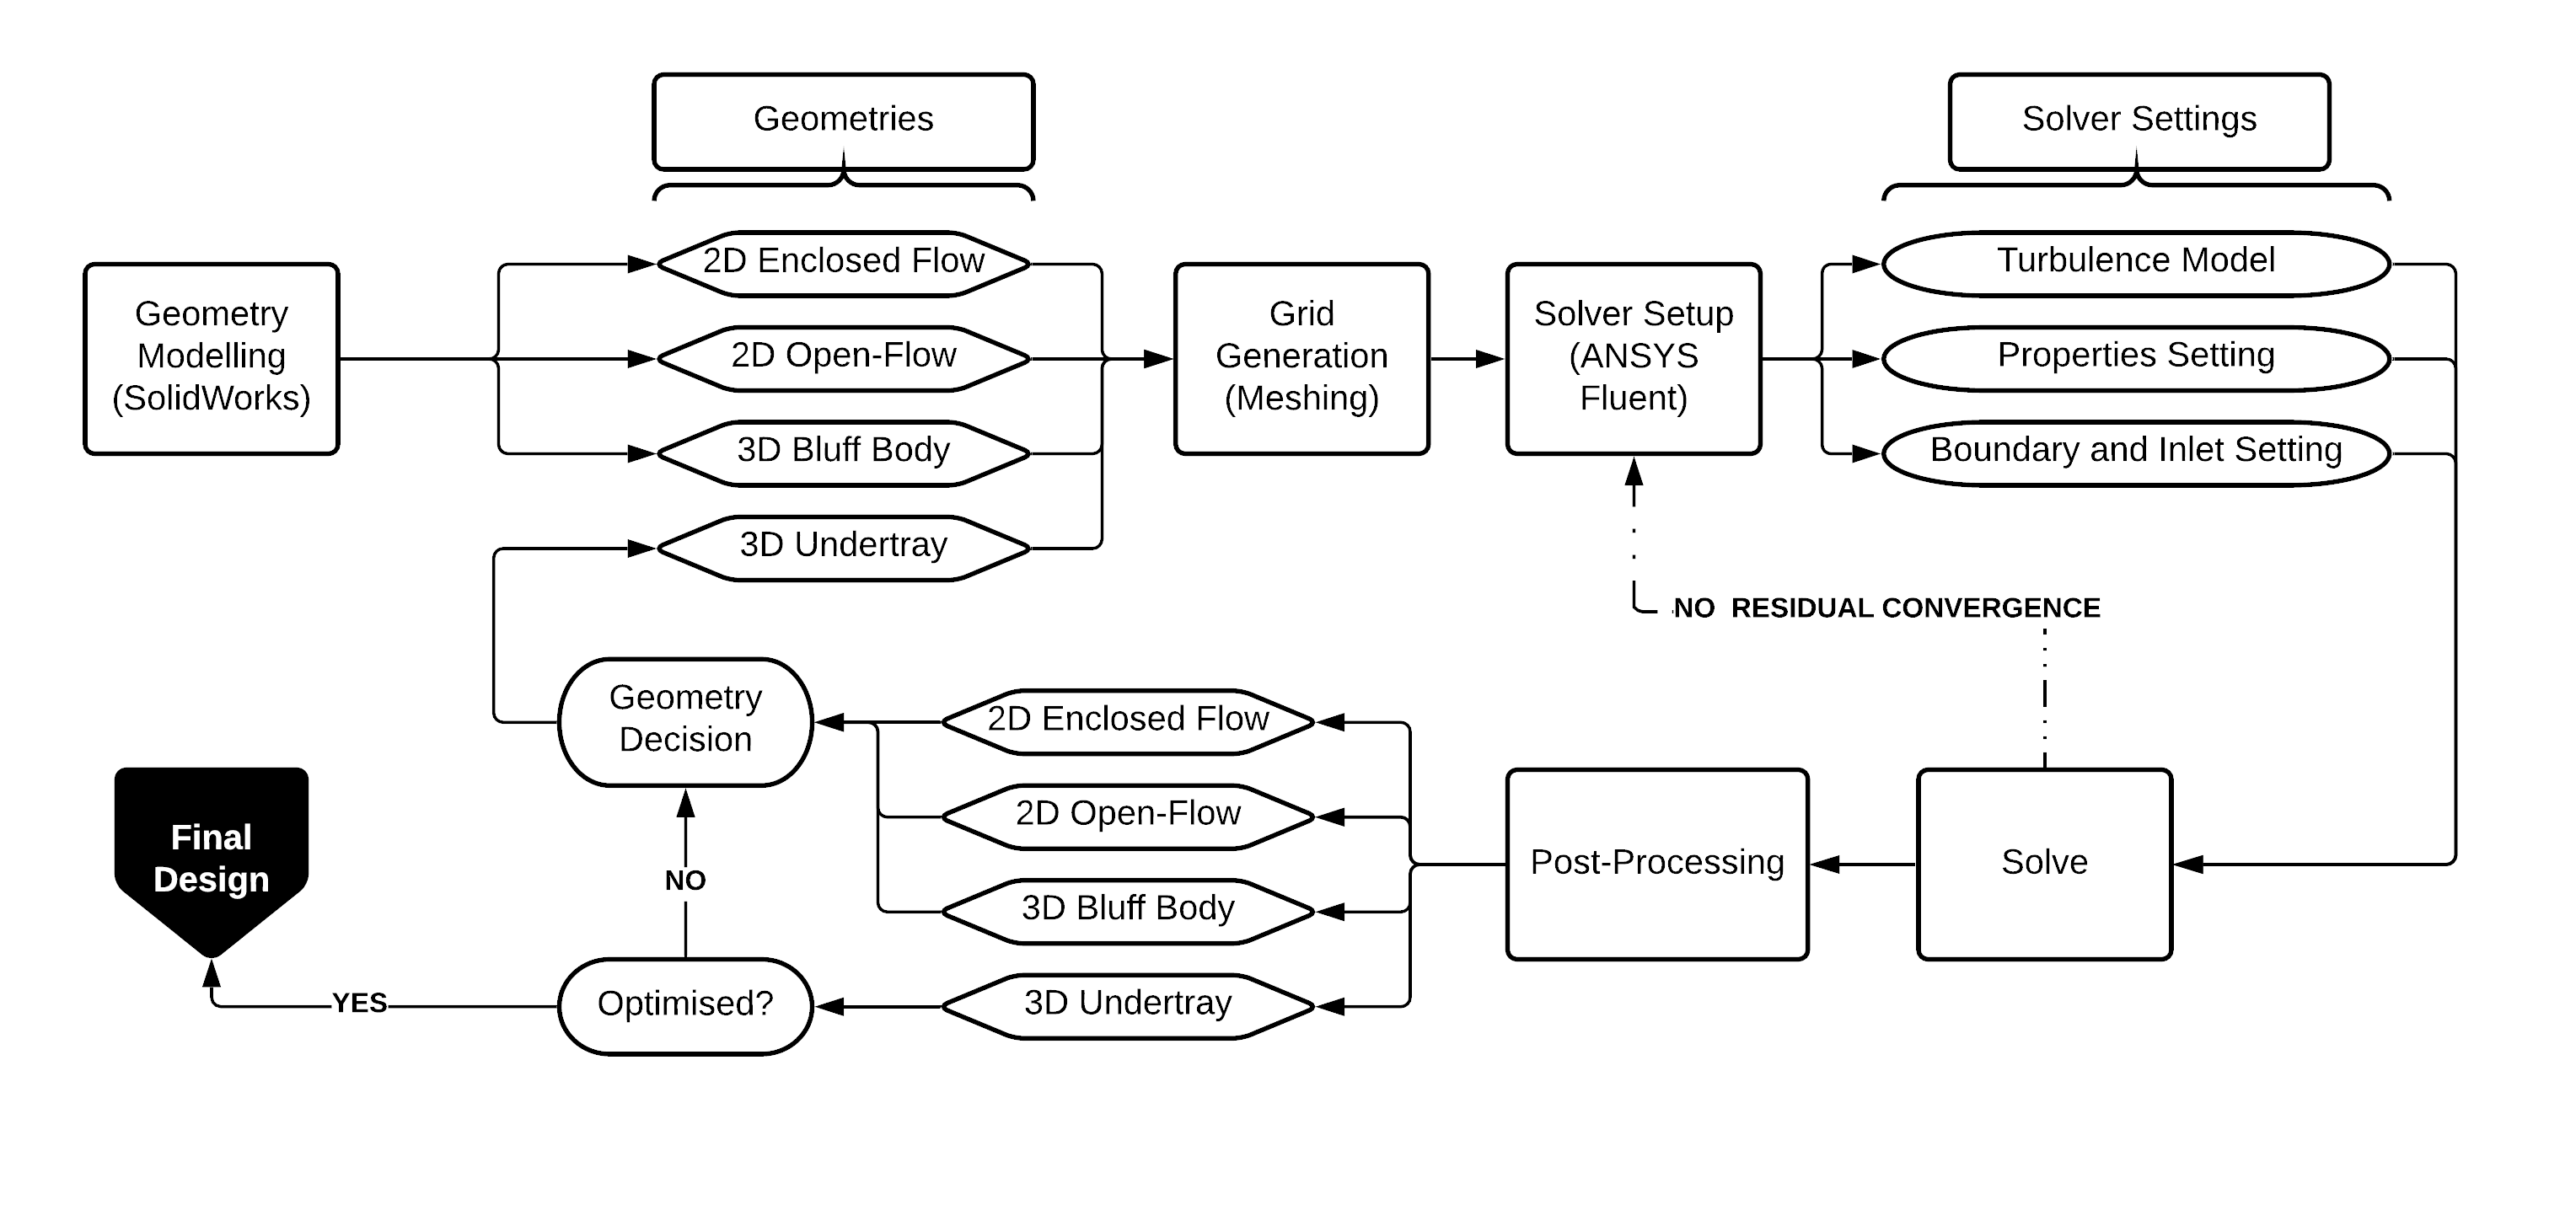
\includegraphics[scale=0.17]{Figures/project_methodology_chart.png}}
    \caption{Project Methodology Flow Chart}
    \label{fig:project methodology}
\end{figure}

\subsection{Pre-Processing \& Solver Setup}

\subsubsection{Grid Generation (Meshing)}
The surface or body which have been defined from SolidWorks becomes the basis for the meshing. Meshing app which integrated in ANSYS workbench provide a user-friendly, simple, and fast meshing generator. Due to the constrain of computational power and time, unstructured triangular (2D) and tetrahedral (3D) mesh were widely used with quadrilateral (2D) and triangular prism (3D) near the wall as an inflation layer to capture the growth of boundary layer and reduce numerical diffusion \cite{Lanfrit2005BestFLUENT}.

\noindent Looking back to the goal of the 2D and 3D bluff body simulation is to obtain and analyse the trend in geometry changes of an undertray, therefore, a non-detailed yet decent mesh could be generated. Local refinement around the body that affected by the fluid flow is recommended \cite{Lanfrit2005BestFLUENT} to achieve a reasonable results and flow representation especially around the undertray, moreover this technique allows larger mesh on the far field section less likely be affected or affecting the result. Other aspect of reasonable meshing is to be aware of the mesh properties such as skewness and growth ratio. For automotive application, it is recommended to have skewness less then 0.45 and maximum growth rate less than 20\% \cite{Lanfrit2005BestFLUENT}. 

\noindent One crucial facet of an undertray flow is generation of boundary layer and how it interacts with the moving floor, the accuracy of this aspect is depend on the quality of layer grid growth near the wall or wall function. To generate a good inflation layer, it is important to make sure the y+ value (first layer height grid) does not exceed the inner boundary layer region which can be done using the equation:

\begin{equation}
    y^+ = \frac{\rho U_\tau \partial y}{\mu}, where \quad U_\tau = \sqrt{\frac{\tau_w}{\rho}} = U \sqrt{\frac{1}{2}C_f}
\end{equation}

\noindent Figure \ref{fig:inflation layer} shows the illustration of y+ value on a wall function. The turbulence model on the solver also has to be a consideration in defining the y+ value, some turbulence modelling require a very low n y+ and some are able to tolerate high y+ value. Detail regarding y+ value in various turbulent model will be discussed on the next section. 

\begin{figure}[!ht]
    \centering
    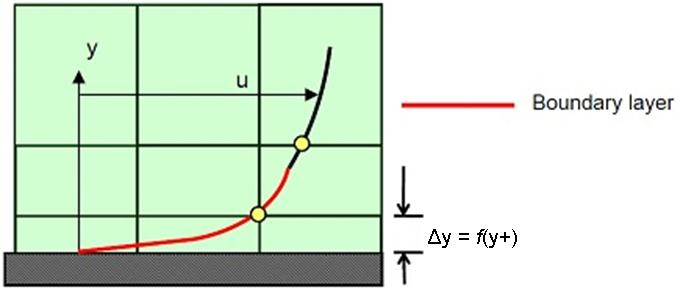
\includegraphics[height=4cm]{Figures/inflation_layer.jpg}
    \caption{Representation of y+ on a near wall function \cite{Anonymous2013Inflate4Blog}}
    \label{fig:inflation layer}
\end{figure}



\subsection{Boundary Conditions}

\begin{table}[!ht]
    \centering
    \caption{Boundary Conditions for 2D and 3D ANSYS Fluent setup}
    \label{tab:Boundary Conditions}
    \vspace{-0.5cm}
\begin{center}
\begin{tabular}{||p{4cm}|p{4cm}|p{7cm}||}
 \hline
 Named Region & Boundary Condition & Property Details\\
 \hline \hline
 \multicolumn{3}{||c||}{General Properties} \\
 \hline
 
 Inlet & Inlet velocity & Velocity = 16.667 m/s (or 40 km/h)\\
 \hline
 Outlet & Outlet Pressure  & Pressure = 101325 Pa  \\
 \hline
 Undertray (2D Enclosed)/Bluff Body & Stationary Wall & No-slip condition\\
 \hline
 Moving Floor & Moving Wall & Velocity = 16.667 m/s (or 40 km/h) in the flow direction\\
 \hline
 Enclosure &   Fluid (Air)  & Pressure = 101325 Pa
Temperature = 288.15 K
Density = 1.225 kg/m3
ISA Sea Level Condition\\
 
 \hline
 \multicolumn{3}{||c||}{3D analyses} \\
 \hline
 
 Symmetry Top & Symmetry  & -\\
 \hline
 Symmetry Side & Symmetry & -\\
 \hline
 
\end{tabular}
\end{center}
\end{table}

\subsection{Numerical Method}



